\newcommand{\econtexRoot}{.}
% The \commands below are required to allow sharing of the same base code via Github between TeXLive on a local machine and Overleaf.  This is an ugly solution to the requirement that custom LaTeX packages be accessible, and that Overleaf seems to ignore symbolic links (even if they are relative links to valid locations)
\providecommand{\econtex}{./texmf-local/tex/latex/econtex}
\providecommand{\econtexSetup}{./texmf-local/tex/latex/econtexSetup}
\providecommand{\econtexShortcuts}{./texmf-local/tex/latex/econtexShortcuts}
\providecommand{\econtexBibMake}{./texmf-local/tex/latex/econtexBibMake}
\providecommand{\econtexBibStyle}{./texmf-local/bibtex/bst/econtex}
\providecommand{\notes}{./texmf-local/tex/latex/handout}
\providecommand{\handoutSetup}{./texmf-local/tex/latex/handoutSetup}
\providecommand{\handoutShortcuts}{./texmf-local/tex/latex/handoutShortcuts}
\providecommand{\handoutBibMake}{./texmf-local/tex/latex/handoutBibMake}
\providecommand{\handoutBibStyle}{./texmf-local/bibtex/bst/handout}

  
\documentclass[titlepage]{\econtex}\providecommand{\texname}{KrusellSmithRep}% Indicate the keyname for the bibtex entry corresponding to this paper
% 2018-10-20: Revise to allow use of either Mathematica or HARK figures (to use Mma figs, comment out the second \FigDir

% 2016-01-30: Fix compilation errors to generate new version; update date on title page
% Modified on 2012/04/21 to fix typo found by Patrick Toche
% Modified by CDC to incorporate edits and insights from Jiaxiong Yao, 2012-08-31


\providecommand{\EqDir}{Equations}
\providecommand{\FigDir}{Figures}
\providecommand{\CodeDir}{Code}
%\providecommand{\CalibrationDir}{Calibration}
\providecommand{\TableDir}{./Tables}
\providecommand{\ApndxDir}{./}

\usepackage{subfiles}
% Now create commands to allow different execution depending on whether compiling main file or subfile            
\newcommand{\onlyinsubfile}[1]{#1}\newcommand{\notinsubfile}[1]{} % https://en.wikibooks.org/wiki/LaTeX/Modular_Documents#Subfiles
\notinsubfile{\immediate\write18{echo \texname > \texname.bibkey}} 

\renewcommand{\FigDir}{./Code/Python/Figures}
\usepackage{\econtexSetup}\usepackage{\econtexShortcuts}

\provideboolean{Shorter}
\setboolean{Shorter}{true}
\providecommand{\ShorterYN}{\ifthenelse{\boolean{Shorter}}}
\usepackage{rotating}\usepackage{subfigure}

\hypersetup{pdfauthor={Tao. Wang <twang80@jhu.edu>},
            pdftitle={Replication of Krusell and Smith(1998)},
            pdfkeywords={Heterogeneous Agents, Wealth Distribution, Marginal Propensity to Consume},
            pdfcreator = {twang80@jhu.edu}
}

\begin{document}\bibliographystyle{\econtexBibStyle}
% Create commands to allow different execution depending on whether compiling main file or subfile            
\renewcommand{\onlyinsubfile}[1]{}\renewcommand{\notinsubfile}[1]{#1} % https://en.wikibooks.org/wiki/LaTeX/Modular_Documents#Subfiles

\hfill{\tiny \texname.tex}

\begin{verbatimwrite}{\texname.title}
Theoretical Foundations of Buffer Stock Saving
\end{verbatimwrite}


\title{Replication of Krusell and Smith(1998)}

\author{Tao Wang \authNum,
Timothy Munday \authNum}

\keywords{Heterogeneous Agents, Wealth Distribution, Marginal Propensity to Consume}

\jelclass{D81, D91, E21}

\maketitle

%\maketitleWithForcedDate{Dec, 2018}


\begin{abstract}
  This paper replecates the work by \cite{krusell1998income} using HARK toolkit. 
\end{abstract}

\begin{small}
\parbox{\textwidth}{
\begin{center}
\begin{tabbing}
\texttt{~Archive:~} \= \= \url{http://github.com/iworld1991/Methods-Project} \kill \\  %
\texttt{~~~~~PDF:~} \> \> \url{http://github.com/iworld1991/Methods-Project/KrusellSmithRep.pdf}    \\
\texttt{~~Github:~} \> \> \url{http://github.com/iworld1991/Methods-Project} \\
\texttt{~~Notebook:~} \> \> \url{http://github.com/iworld1991/Methods-Project/KrusellSmith.ipynb} 

\end{tabbing}
\end{center}
}
\end{small}

% \begin{comment}

\begin{authorsinfo}
\name{Contact: \href{mailto:twang80@jhu.edu}{\texttt{twang80@jhu.edu}}, Department of Economics, 590 Wyman Hall, Johns Hopkins University, Baltimore, MD 21218, \url{http://taowangecon.github.io}.}
\end{authorsinfo}
%\end{comment}

\thanks{Great thanks to Chris Carroll for editing of the draft notebook and Matthew White for the insightful and detailed explanation of HARK.}

\titlepagefinish

%\large\opt{FromShell}{\normalsize} %

\newtheorem{defn}{Definition}
\newtheorem{theorem}{Theorem}

\section{Introduction}

\label{sec:intro}

This is an introduction. Including motivation, overview of the paper, etc. 

The benchmark Krusell-Smith model has the following broad features:

\begin{itemize}
\item The aggregate state switches between "good" and "bad" with known probabilities
\item  All consumers experience the same aggregate state for the economy (good or bad)
\item Ex ante there is only one type of consumer, which is infinitely lived
\item  Ex post heterogeneity arises from uninsurable idiosyncratic income shocks
\item Specifically, individuals are at risk of spells of unemployment
\item In a spell of unemployment, their income is zero
\end{itemize}
Thus, each agent faces two types of uncertainty: About their employment state, and about the income they will earn when employed.  And the values of income and unemployment risk depend on the aggregate state.

\section{Model}

\subsection{Setup}

\textbf{Individual Agents}

Each agent  attempts  to supply an amount of productive labor $\ell$ in each period. 

However, whether they succeed in supplying that labor (and earning a corresponding wage) is governed by the realization of the stochastic variable $\epsilon$.  If the agent is unlucky, $\epsilon$ is zero and the agent is unemployed.  The amount of labor they succeed in supplying is thus $\epsilon\ell$.

Therefore, a consumer's income is the following.

\begin{eqnarray}
y & = & w p \ell \epsilon 
\end{eqnarray}

where $p$ is the persistent component of income.  Krusell and Smith did not incorporate a persistent component of income, however, so we will simply calibrate $p=1$ for all states.

For each of the two aggregate states we need to specify:
\begin{itemize}
\item The proportion of consumers in the $e$ and the $u$ states
\item The level of persistent/permanent productivity $p$ (always 1)
\item The ratio of actual to permanent productivity in each state $\{e,u\}$
\item In the KS notation, this is $\epsilon\ell$  
\end{itemize}


\textbf{Aggregate Economy}

Aggregate output ($\bar{y}$) is produced using a Cobb-Douglas production function using capital and labor. (Bars over variables indicate the aggregate value of a variable that has different values across different idiosyncratic consumers).

$z$ denotes the aggregate shock to productivity. $z$ can take two values, either $z_g$ -- the "good" state, or $z_b < z_g$ -- the "bad" state.  Consumers gain income from providing labor, and from the rental return on any capital they own.  Labor and capital markets are perfectly efficient so both factors are both paid their marginal products.

The agent can choose to save by buying capital $k$ which is bounded below at the borrowing constraint of 0.

Putting all of this together, aggregate output is given by 

\begin{verbatimwrite}{\EqDir/cbprod.tex}
\begin{eqnarray}
  \label{eq:cbprod}
\bar{y} & = & z\bar{k}^\alpha \bar{\ell}^{1-\alpha}
\end{eqnarray}
\end{verbatimwrite}

\begin{eqnarray}
  \label{eq:cbprod}
\bar{y} & = & z\bar{k}^\alpha \bar{\ell}^{1-\alpha}
\end{eqnarray}


The aggregate shocks $z$ follow a first-order Markov chains with the transition probability of moving from state $s$ to state $s'$ denoted by $\pi_{ss'}$. The aggregate shocks and individual shocks are correlated: The probability of being unemployed is higher in bad times, when aggregate productivity is low, than in good times, when aggregate productivity is high.

There are restrictions as to how the aggregate and idiosyncratic shocks are correlated. 

$\forall \{s,s'\}=\{g,b\}\times\{g,b\}$, the following two conditions hold:

$$\underbrace{\pi_{ss'01}}_{p(s \rightarrow s',u \rightarrow e)}+\underbrace{\pi_{ss'00}}_{p(s \rightarrow s', u \rightarrow u)} = \underbrace{\pi_{ss'11}}_{p(s\rightarrow s', e \rightarrow e) }  + \underbrace{\pi_{ss'10}}_{p(s \rightarrow s', e \rightarrow u)} = \underbrace{\pi_{ss'}}_{p(s\rightarrow s')}$$

$$u_s \frac{\pi_{ss'00}}{\pi_{ss'}}+ (1-u_s) \frac{\pi_{ss'10}}{\pi_{ss'}} = u_{s'}$$

\textbf{Individuals and Aggregate Economy}

The individual shocks satisfy the law of large numbers, and the model is constructed so that the number of agents who are unemployed in the good state always equals $u_g$, and is always $u_b$ in the bad state. Given the aggregate state, individual shocks are independent from each other.

For the individual, the probability of moving between a good state and employment to a bad state and unemployment is denoted $\pi_{gb10}$ with similar notation for the other transition probabilities.

(Krusell and Smith allow for serially correlated unemployment at the idiosyncratic level. Here we will simplify this and have unemployment be serially uncorrelated.)

Finally, $\Gamma$ denotes the current distribution of consumers over capital and employment status, and $H$ denotes the law of motion of this distribution. 

\textbf{Individual's Problem Given Aggregate State}

The individual's problem is:
\begin{eqnarray*}
	V(k, \epsilon; \Gamma, z) &=& \max_{k'}\{U(c) + \beta \mathbb{E}[V(k' ,\epsilon'; \Gamma', z')|z, \epsilon]\} \\
	c + k' &=& r(\bar{k}, \bar{\ell}, z)k + w(\bar{k}, \bar{\ell}, z)\ell\epsilon + (1-\delta)k \\
	\Gamma' &=& H(\Gamma, z, z') \\
	k' &\geq& 0 \\
\end{eqnarray*}

Krusell and Smith define an equilibrium as a law of motion $H$, a value function $V$, a rule for updating capital $f$ and pricing functions $r$ and $w$, such that $V$ and $f$ solve the consumers problem, $r$ and $w$ denote the marginal products of capital and labour, and $H$ is consistent with $f$ (i.e. if we add up all of the individual agents capital choices we get the correct distribution of capital).

\section{Algorithm}

In principle, $\Gamma$ is a high-dimensional object because it includes the whole distribution of individuals' wealth in the economy. Because the optimal amount to save is a nonlinear function of the level of idiosyncratic $k$, next period's aggregate capital stock $\bar{k}'$ depends on the distribution of the holdings of idiosyncratic $k$ across the population of consumers. Therefore the law of motion $H$ is not a trivial function of the $\Gamma$. 

KS simplified this problem as by noting the following. 

\begin{enumerate}
\item The agent cares about the future aggregate aggregate state only insofar as that state affects their own personal value of $c$
\item Future values of $c$ depend on the aggregate state only through the budget constraint
\item The channels by which the budget constraint depends on the aggregate state are:
\begin{itemize}
\item The probability distributions of $\epsilon$ and $z$ are affected by the aggregate state
\item Interest rates and wages depend on the future values of $\bar{k}$ and $\bar{\ell}$
\end{itemize}
\item The probability distributions for the future values of $\{\epsilon, z\}$ are known
\begin{itemize}
	\item They are fully determined by the Markov transition matrices
\end{itemize}
\item But the values of $r$ and $w$ are both determined by the future value of $\bar{k}$ (in combination with the exogenous value of $\bar{\ell}$)
\begin{itemize}
	\item  So the only endogenous object that the agent needs to form expectations about, in order to have a complete rational expectation about everything affecting them, is $\bar{k}'$
\end{itemize}
\end{enumerate}
The key result in Krusell and Smith is the discovery that a very simple linear rule does an extraordinarily good job (though not quite perfect) in forecasting $\bar{k'}$

They then argue that, since rationality is surely bounded to some degree, the solution that an agent obtains using a good forecasting rule for $\bar{k}'$ is "good enough" to compute an "approximate" solution to the consumer's optimization problem.

They define a generic algorithm to find a forecasting rule for $\bar{k}$ as follows

\begin{enumerate}
	\item  Choose the number of moments $n$ of the distribution of $k$ to be included in the set of variables to forecast $\bar{k}'$. In the simplest case, $n=1$, the only forecasting variable for next period's $\bar{k}'$ is the mean (the first moment, $n=1$)) of current capital, $\bar{k}$.
	\item Each individual adopts the same belief about the law motion of these moments, $H_I$ and finds the optimal decision policy, $f_I$, contingent on that guess.
	\item Use the optimal policy to simulate a history of aggregate capital with a large number of agents. 
	\item Characterize the realized law of motion using the same number of moments $n$ 
	\item Compare it with the $H_I$, what is taken as given by individuals. 
	\item Iterate until the two converge. 
\end{enumerate}

In the end, the solution to the original problem is well approximated by the following simplified problem:

\begin{eqnarray*}
	V(k, \epsilon; \bar k, z) &=& max_{c, k'}\{U(c) + \beta E[V(k' ,\epsilon'; \bar k', z')|z, \epsilon]\} \\
	c + k' &=& r(\bar{k}, \bar{\ell}, z)k + w(\bar{k}, \bar{\ell}, z)l\epsilon + (1-\delta)k \\
	\text{When }~ z=z_g, \quad \mathbb{E}[\log\bar{k}'] & = & a_0 + a_1 \log\bar k \\
	\text{When }~ z=z_b,  \quad \mathbb{E}[\log\bar{k}'] & = & b_0 + b_1 \log\bar k \\
	k' &\geq& 0 \\
\end{eqnarray*}

\section{Parameterization}

The parameters of the model are given in Table \ref{table:parameters}.

\begin{table}
\begin{center}
\caption{Parameters of Krusell and Smith}\label{table:parameters}
\begin{tabular}{|c|c|c|}
\hline 
Description                     & \multicolumn{1}{c}{Parameter} & Value  \\ \hline
\multicolumn{3}{|c|}{Individual Parameters}  \\ \hline
Time Preference Factor          & \multicolumn{1}{c}{$\beta$} & 0.99  \\
Coefficient of Relative Risk Aversion & \multicolumn{1}{c}{$\CRRA$} & 1.0  \\
Transition Probability of Macroeconomic State  & \multicolumn{1}{c}{$\pi_{ss'}$} & 0.175 \\
Probability of Unemployment in Good State  & \multicolumn{1}{c}{$u_g$} & 0.040 \\
 Probability of Unemployment in Bad State  & \multicolumn{1}{c}{$u_b$} & 0.100 \\
 \hline 
 \multicolumn{3}{|c|}{Macroeconomic Parameters}  \\ 
 \hline
 Capital Share of the Production Function & \multicolumn{1}{c}{$\alpha$} & 0.330 \\
 Depreciation Factor & \multicolumn{1}{c}{$\delta$} & 0.025 \\
 Productivity in Good State & \multicolumn{1}{c}{$z_g$} & 1.01 \\
 Productivity in Bad State & \multicolumn{1}{c}{$z_b$} & 0.99 \\
\hline
\end{tabular}
\end{center}
\end{table}


\section{Results}

\subsection{Consumption Function and Evolution of Aggregate Capital}

The consistent law of motion of aggregate capital in good and bad states are as below. 


\begin{eqnarray*}
	\text{When }~ z=z_g, \quad \mathbb{E}[\log\bar{k}'] & = & -0.078 + 0.995 \log\bar k, \quad R^2 = 0.999999\\
	\text{When }~ z=z_b,  \quad \mathbb{E}[\log\bar{k}'] & = & -0.077 + 0.995 \log\bar k, \quad R^2 = 0.999999\\
\end{eqnarray*}

Graphically, the aggregate capital evolves as shown in Figure \ref{fig:kfunc}.
 
\begin{figure}[tbp]
	\centerline{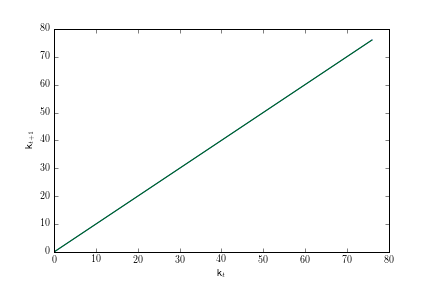
\includegraphics[width=4in]{\FigDir/KFuncsConverge.png}}
	\caption{Aggregate Saving as a Function of Aggregate Market Resources}
	\label{fig:kfunc}
\end{figure}

Figure \ref{fig:cfunc} plots the individual consumption as a function of individual market resourses. Each line in the graph represents a different level of aggregate capital. 

\begin{figure}[tbp]
	\centerline{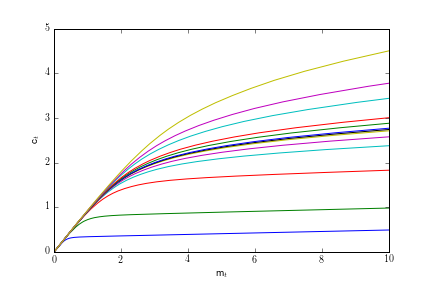
\includegraphics[width=4in]{\FigDir/cFuncsConverge.png}}
	\caption{Individual Consumption Function at Different Levels of Aggregate Capital}
	\label{fig:cfunc}
\end{figure}

Figure \ref{fig:sfunc} plots the individual saving as a function of individual market resourse.  

\begin{figure}[tbp]
	\centerline{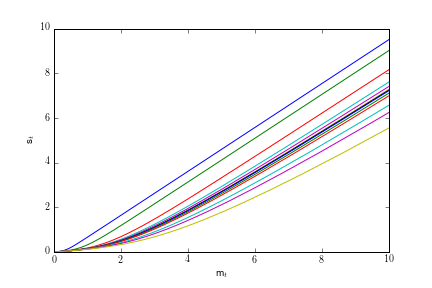
\includegraphics[width=4in]{\FigDir/sFuncsConverge.png}}
	\caption{Individual Saving Function at Different Levels of Aggregate Capital}
	\label{fig:sfunc}
\end{figure}


\subsection{Wealth Distribution}

\subsubsection{Baseline}

The wealth distribution in steady state of the baseline model is shown in Figure \ref{fig:lorenzbaseline}.

\begin{figure}[tbp]
	\centerline{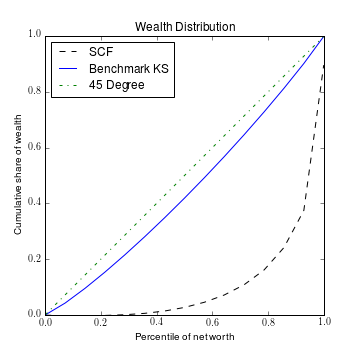
\includegraphics[width=4in]{\FigDir/LorenzBaseline.png}}
	\caption{Wealth Distribution in Baseline Krusell Smith}
	\label{fig:lorenzbaseline}
\end{figure}


\subsubsection{Heterogeneous Time Preferences}


As the Figure \ref{fig:lorenzbaseline} shows, the distribution of wealth that the baseline KS model produces is very far from matching the empirical degree of inequality in the US data.

This could matter for macroeconomic purposes.  For example, the SCF data indicate that many agents are concentrated at low values of wealth where the MPC is very large.  We might expect, therefore, that a fiscal policy "stimulus" that gives a fixed amount of money to every agent would have a large effect on the consumption of the low-wealth households who have a high Marginal Propensity to Consume.


\begin{figure}[tbp]
	\centerline{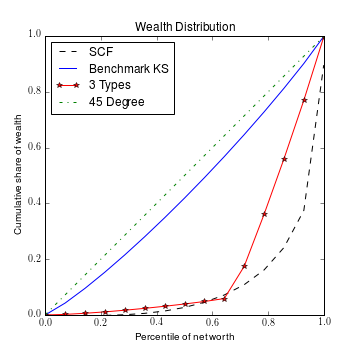
\includegraphics[width=4in]{\FigDir/Lorenz3beta.png}}
	\caption{Wealth Distribution in Baseline Krusell Smith}
	\label{fig:lorenz3beta}
\end{figure}


KS attempt to address this problem by assuming that an individual agent's time preference rate can change over time.

The rationale is that this represents a generational transition: The "agent" is really a "dynasty" and the time preference rate of the "child" dynast may differ from that of the ``parent.''

Specifically, KS assume that $\beta$ can take on three values, 0.9858, 0.9894, and 0.9930, and that the transition probabilities are such that 

\begin{enumerate}
	
\item The invariant distribution for $\beta$'s has 80 percent of the population at the middle $\beta$ and 10 percent at each of the other $\beta$'s.
\item Immediate transitions between the extreme values of $\beta$ occur with probability zero. 
\item The average duration of the highest and lowest $\beta$'s is 50 years. 
\end{enumerate}

The HARK toolkit is not natively set up to accommodate stochastic time preference factors (though an extension to accommodate this would be easy).  

Here, instead, we assume that different agents have different values of $\beta$ that are uniformly distributed over some range. We approximate the uniform distribution by three points.  The agents are heterogeneous ex ante (and permanently).

The results are plotted in Figure \ref{fig:lorenz3beta}. Notice that now by allowing heterogeity in time preferences, we are able to match the wealth inequality observed from consumers' data better.  

\section{Concluding Remarks}

This is a section for conclusion. 

%\clearpage\vfill\eject

\normalsize

% This is for robustness; if these files don't exist, bibtex will get mad
%\write18{if [ ! -f \texname.bib     ]; then touch \texname.bib     ; fi}
%\write18{if [ ! -f \texname-Add.bib ]; then touch \texname-Add.bib ; fi}

\bibliography{KrusellSmithRep,\texname,\texname-Add}

\end{document}
